

\documentclass[a4paper,doc,natbib,floatsintext]{apa6}\usepackage[]{graphicx}\usepackage[]{color}
%% maxwidth is the original width if it is less than linewidth
%% otherwise use linewidth (to make sure the graphics do not exceed the margin)
\makeatletter
\def\maxwidth{ %
  \ifdim\Gin@nat@width>\linewidth
    \linewidth
  \else
    \Gin@nat@width
  \fi
}
\makeatother

\definecolor{fgcolor}{rgb}{0.345, 0.345, 0.345}
\newcommand{\hlnum}[1]{\textcolor[rgb]{0.686,0.059,0.569}{#1}}%
\newcommand{\hlstr}[1]{\textcolor[rgb]{0.192,0.494,0.8}{#1}}%
\newcommand{\hlcom}[1]{\textcolor[rgb]{0.678,0.584,0.686}{\textit{#1}}}%
\newcommand{\hlopt}[1]{\textcolor[rgb]{0,0,0}{#1}}%
\newcommand{\hlstd}[1]{\textcolor[rgb]{0.345,0.345,0.345}{#1}}%
\newcommand{\hlkwa}[1]{\textcolor[rgb]{0.161,0.373,0.58}{\textbf{#1}}}%
\newcommand{\hlkwb}[1]{\textcolor[rgb]{0.69,0.353,0.396}{#1}}%
\newcommand{\hlkwc}[1]{\textcolor[rgb]{0.333,0.667,0.333}{#1}}%
\newcommand{\hlkwd}[1]{\textcolor[rgb]{0.737,0.353,0.396}{\textbf{#1}}}%

\usepackage{framed}
\makeatletter
\newenvironment{kframe}{%
 \def\at@end@of@kframe{}%
 \ifinner\ifhmode%
  \def\at@end@of@kframe{\end{minipage}}%
  \begin{minipage}{\columnwidth}%
 \fi\fi%
 \def\FrameCommand##1{\hskip\@totalleftmargin \hskip-\fboxsep
 \colorbox{shadecolor}{##1}\hskip-\fboxsep
     % There is no \\@totalrightmargin, so:
     \hskip-\linewidth \hskip-\@totalleftmargin \hskip\columnwidth}%
 \MakeFramed {\advance\hsize-\width
   \@totalleftmargin\z@ \linewidth\hsize
   \@setminipage}}%
 {\par\unskip\endMakeFramed%
 \at@end@of@kframe}
\makeatother

\definecolor{shadecolor}{rgb}{.97, .97, .97}
\definecolor{messagecolor}{rgb}{0, 0, 0}
\definecolor{warningcolor}{rgb}{1, 0, 1}
\definecolor{errorcolor}{rgb}{1, 0, 0}
\newenvironment{knitrout}{}{} % an empty environment to be redefined in TeX

\usepackage{alltt}
\usepackage[english]{babel}
\usepackage[utf8x]{inputenc}
\usepackage{amsmath}
\usepackage{graphicx}
\usepackage{rotating}
\usepackage{pdfpages}
%\usepackage{Sweave}
\usepackage{subcaption}
\usepackage{float}
\usepackage{eurosym}
%\SweaveOpts{concordance=TRUE}

\graphicspath{{articles/article1/}}

\title{Peeks and Keeps: A new paradigm to study the exploration-exploitation trade-off}
\shorttitle{peeks and keeps}
\twoauthors{Nathaniel D. Phillips and Hans Joerg Neth}{Daniel Navarro}
\twoaffiliations{University of Konstanz}{University of Adelaide}

\abstract{Many important decision tasks involve an exploration-exploitation trade-off, where organisms have the competing goals of gaining new information (exploration) to improve future decisions, and acting on existing information (exploitation). The most common paradigm to study this trade-off experimentally is the n-armed bandit, where decision makers reap real costs and rewards on every trial. We suggest that, unlike the n-armed bandit, many real world tasks allow decision makers to explore options (such as stock price changes) without reaping any costs or rewards. To address this, we introduce a new experimental paradigm called ``Peeks and Keeps'' that combines aspects of the n-armed bandit with the `bet-observe' task \citep{tversky1966information}. Unlike the n-armed bandit, Peeks and Keeps gives decision makers the option of explicitly separating exploration and exploitation behavior, where exploration provides only information but no costs or rewards, and exploitation gives both information and costs and rewards. This paradigm not only increases the empirical validity of the n-armed bandit, but also provides researchers with an explicit measure of exploration that is hidden in other paradigms.}

\keywords{decisions from experience, learning, information search, exploration-exploitation, foraging}
\IfFileExists{upquote.sty}{\usepackage{upquote}}{}
\begin{document}


% (purely) epistemic vs. pragmatic
% theoretical vs. practical
% no consequence vs. consequence


\maketitle

\section{Exploration-exploitation trade-off}

Many of the most important real world decisions require individuals to reap consequences from several risky options that probabilistically give rewards and punishments. In many tasks, these decisions are made under uncertainty, where the probabilities and magnitudes associated with options are \textit{a priori} unknown. In order to learn about options, organisms can engage in active search which improves the quality of their impressions of options. However, search can come at a cost, such as the missed opportunity to receive rewards from known options. For example, in trying a new restaurant, one forgoes the opportunity to have a meal at her (current) favorite restaurant.

This conflict between obtaining new information and acting on existing information is known as the exploration-exploitation trade-off. The exploration-exploitation (EE) trade-off is one of the most widely studied aspects of decision making from human to non-human organisms. The exploration-exploitation trade-off represents a goal conflict in decisions under uncertainty, where an organism is trying to maximize its long term rewards from \textit{a priori} unknown options. On the one hand, individuals want to explore options by gaining as much information as possible to improve the quality of their future decisions. On the other hand, they want to \textit{exploit} options by acting on existing information in order to increase short-term rewards.

One of the most widely used experimental tasks used to study the exploration-exploitation conflict is the n-armed bandit. In an n-armed bandit, participants have a fixed number of trials to select an option and experience a consequential reward.



\subsection{Purely epistemic versus pragmatic actions}

\begin{itemize}

  \item \cite{neth2008thinking} distinguished between two types of actions, epistemic and pragmatic. Epistemic actions are those that result in information rather than punishments or rewards, while pragmatic actions are those that lead to punishments or rewards. Exploration is assumed to be an epistemic action while exploitation is a pragmatic action.
  
  \item One can easily imagine real-world cases where people explicitly engage in purely epistemic actions. For example, imagine a person who wishes to learn about the stock market prior to risking any real money. He can do this by viewing sequential returns from several stocks and observing their risk. Alternatively, a new resident to a town can learn about local restaurants by asking her neighbors about their recent experiences. In all of these cases, the actor is learning about options without reaping consequences.
  
  \item Clearly these purely epistemic actions are both psychologically and behaviorally distinct from pragmatic actions, where one obtains \textit{both} information and immediate consequences. For example, our stock investor who starts investing his money into stocks will then not only learn about their performance, but also reap gains and suffer consequences. Similarly, the new town resident who starts frequenting local restaurants will continue learning about them but also experience immediate pragmatic outcomes.
  
  \item Somewhat puzzlingly, paradigms that have been used to study exploration-exploitation trade-off in humans has largely ignored behavioral differences in epistimic and pragmatic actions. In the N-armed bandit task, players are only allowed to engage in one type of behavior - choice, which always provides both epistemic and pragmatic rewards. Players are not given the option to engage in purely epistemic actions. 
  
  \item This can lead to erroneous inferences. The same choice behavior could be interpreted as either resulting from an epistemic or pragmatic motivation. Until now, researchers have had to use computational cognitive modeling techniques to attribute choices post-hoc to either an epistemic or pragmatic underlying goal.
  
  \item We believe a new paradigm is needed. One where individuals have the option to explicitly explore or exploit options. This task will not only be a better model of many real-world decision tasks than previous paradigms, but will also allow researchers to explicitly observe behavior consistent with purely epistemic goals.

\end{itemize}

\subsection{Combining three paradigms}


\begin{center}
    \begin{tabular}{ | l | l | l | l | l |}
    \hline
    Paradigm & EE Tradeoff & Pure Exploration & Pure Exploitation & Alternation \\ \hline
    N-Armed Bandit & Yes & No & No & Yes\\ \hline
    Sampling Paradigm & No & Yes & Yes & No\\ \hline
    Bet-Observe & Yes & Yes & Yes & Yes\\ \hline
    Peeks and Keeps & Yes & Yes & No & Yes\\ \hline
    \hline
    \end{tabular}
\end{center}


In a multi-armed bandit task, participants choose between multiple a priori unknown options over several trials and receive rewards (or costs) on each trial. Because decision makers reap consequences on every trial, the n-armed bandit task does not allow purely epidemic actions. The Iowa Gambling Task (IGT) is one famous example of this paradigm. Using cognitive models such as the expectancy-valence model, researchers have used the IGT to study cognitive mechanisms such as loss-aversion, recency, and choice consistency in both healthy and non-healthy individuals \citep{yechiam2005models}.

Two paradigms have been used to study purely epistemic actions: the sampling paradigm of decisions from experience \citep{hertwig2004decisions} and the bet-observe task \citep{tversky1966information}. Like the n-armed bandit task, both paradigms present participants with multiple, a priori unknown options. In the sampling paradigm, participants can then sample from options, without consequence, as many times as they would like before making a single consequential choice. Here, participants engage in a self-determined number of purely epistemic actions strictly prior to a single purely pragmatic action. After making their final choice, participants receive the consequences from their choice but cannot continue to observe. Thus, in the sampling paradigm observation strictly occurs prior to exploitation with no possibility to alternate between the two modes.

As far as we know, the bet-observe task is the only paradigm that allows individuals to alternate between pure exploration and pure exploitation. In the bet-observe task, an individual is presented with two options. On each of M trials, one of the two options will produce a reward indicated by a green light. On each trial, the participant selects an option and makes one of two choices. He can \textit{observe} an option, see which one produces the reward, but not receive the reward. Or he can \textit{bet} on an option. If the player bets on an option, he will gain its underlying reward but will not see whether the reward is present. Because the participant only sees the option outcome if he observes, he can only learn about the options' underlying distributions on observation trials, but can only reap rewards on betting trials.

Navarro and Newell (2014) derived optimal decision strategies for two versions of the game: stationary and non-stationary. In the stationary version of the game, the reward probability distributions are fixed. Specifically, the probability that the left option has a reward $l_{p}$ is fixed and does not change over time. In the stationary task, an optimal learner will begin the task by observing outcomes until he reaches a pre-defined information threshold. Once he reaches this threshold, he will switch to a betting strategy and will always bet on the perceived better option. In the non stationary version of the game, the reward probability distributions can change at any time. For example, with some probability $\alpha$ the probability $l_{p}$ could change to a value drawn from a uniform distribution. In this version of the game, the optimal decision strategy alternates between observing and betting throughout the game. In other words, the actor will begin by observing for a few trials until a certain information threshold is reached, then he will switch to betting for a few trials. He will then switch to observing in order to see if $l_{p}$ has changed.

However, because betting in the bet-observe task does not provide information, decision makers cannot learn anything on betting trials. This is not an inherent flaw in the paradigm - indeed, obscuring information from betting trials elegantly separates epistemic from pragmatic actions. However, because many, if not most, real-world decision tasks provide information on both exploration and exploitation trials, the bet-observe task is a poor model of most real-world decisions. From food choice to mate choice, exploitation decisions (i.e.; consuming food or selecting a mate) will always provide information to the decision maker that it can use to update its impressions and guide future search. 

In order to study how people alternate between explicit exploration and exploitation, we introduce the Peeks and Keeps task.


\section{Peeks and Keeps}

Peeks and Keeps is an extension of an N-armed bandit task that explicitly separates exploration and exploitation decisions. In the task, participants repeatedly select one of N options with \textit{a priori} unknown underlying probability distributions over the course of M trials. On each trial, the participant selects an option and elects to either \textit{observe} the next outcome without financial feedback, or \textit{bet} on the outcome and receive the financial feedback. At the end of M trials, the participant is paid the sum of all sample outcomes revealed on bet trials. If he always observes and never bets, he receives no bonus. If he bets on every trial, he receives the sum total of all samples.

\section{Decision Strategies}

We split cognitive strategies in Peeks and Keeps into three distinct processes: Selection, Action, and Update. The selection process determines which option players interact with, the action process determines whether a player decides to peek or keep, and the updating process dictates how a player updates his or her impressions of that option after the action.

The specific order of these processes depends on the overarching search model. In the SAU Model, we assume that decision makers process information in the order Selection-Action-Update. In the ASU model, we assume that they process information in the order Action-Selection-Update.


\begin{center}
\begin{knitrout}
\definecolor{shadecolor}{rgb}{0.969, 0.969, 0.969}\color{fgcolor}
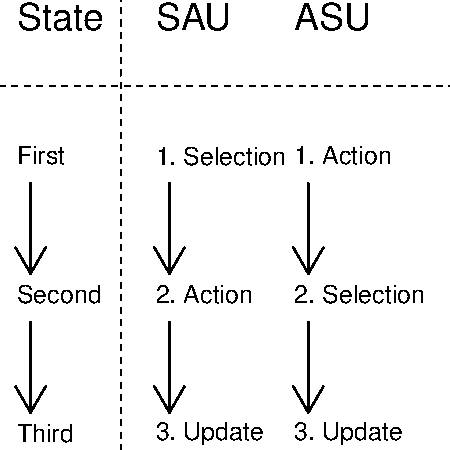
\includegraphics[width=\maxwidth]{figure/unnamed-chunk-1-1} 

\end{knitrout}
\end{center}

In addition to dictating the order of the cognitive processes, the SAU and ASU models each potentially dictate different cognitive processes for each processing step. In the next two sections, we describe potential cognitive processes under each model.

\section{SAU}

The SAU model assumes that decision makers begin by selecting an option, followed by an action decision. Because the SAU model begins with the selection process, the SAU model is most similar to existing cognitive models of search \citep{yechiam2005models}.

\subsection{Selection}

\subsubsection{Soft-Max}

We follow prior research in assuming that people use a soft-max selection rule, where the probability that an option is selected is determined as an increasing function of the expectation of that option relative to the sum of the expectations of all options. Formally:

\begin{center}
\begin{equation}

Pr[G_{j}(t+1)]=\frac{e^{\theta(t) \times E_{j}(t)}}{\sum_{k}e^{\theta(t) \times E_{k}(t)}}


\end{equation}
\end{center}

The term $\theta(t)$ governs how sensitive people are to expectations in directing their selection. We follow previous researchers \citep{yechiam2005models} in setting $\theta(t)$ to be a function of time and a response-sensitivity parameter c

\begin{center}
\begin{equation}
\label{eq:thetat}

\theta(t) = (\frac{t}{n_{t} \times .5})^{c}

\label{eq:softmaxtheta}
\end{equation}
\end{center}

where c has a support of [0, Inf]. As c increases, people more clearly separate their search into distinct exploration and exploitation phases. Small values of c less clear distinction between phases. Because equation \ref{eq:thetat} is a monotonically increasing function of trials, participants are assumed to be increasingly more likely to select options with higher expectations as trials increase\footnote{Note: The curve has an indifference point where the probability of selecting all options is equally likely. In Equation~\ref{eq:softmaxtheta}, the indifference point occurs at half-way through the game (total trials times .50). However, the model could be expanded to allow this indifference point to occur at a different location. Indeed, other authors have hard-coded this indifference point to occur at a trial of 10 \citep{yechiam2005models}}.


\begin{knitrout}
\definecolor{shadecolor}{rgb}{0.969, 0.969, 0.969}\color{fgcolor}
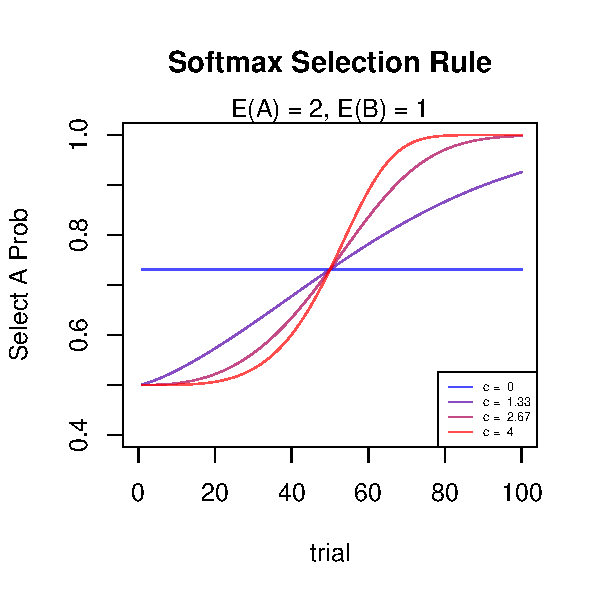
\includegraphics[width=\maxwidth]{figure/unnamed-chunk-2-1} 

\end{knitrout}


\subsection{Action}

Once an option is selected, the decision maker decides whether to peek or keep. We propose three different models that could drive this decision. Each model focuses on a particular statistic of the selected option.

\subsubsection{Probability of a negative outcome}

The first action function predicts that people will keep an option as a decreasing function of the perceived probability that the next outcome will be negative:

\begin{center}
\begin{equation}
\label{eq:actionpneg}

Pr(Keep_{t})= \frac{1}{1 + e^{\alpha \times (\beta_{t} - \gamma)}}

\end{equation}
\end{center}

Each parameter is defined as follows: $\alpha$ falls in the range [0, Inf] and is the sensitivity to differences in perceived probability of negative outcomes. When $\alpha$ is 0, changes in perceived probability of obtaining negative outcomes does not affect action decisions. When $\alpha$ is very large, small differences in the perceived probability of drawing a negative outcome dramatically change action decisions. $\beta_{t}$ falls in the range [0, 1] and is the perceived probability of observing a negative outcome from the selected option at trial t. $\gamma$ falls in the range [-Inf, Inf] and represents is the overall tolerance for keeping negative outcomes. Specifically, $\gamma$ represents the perceived probability of sampling a negative outcome where the decision maker is equally likely to keep or peek. When $\gamma$ is negative, people are always more likely to peek than keep, while when $\gamma$ is greater than 1, people are always more likely to keep than peek.

From this setup, an unbiased agent that always keeps when the perceived probability of a negative value is less than .5, and always peeks when the perceived probability of a negative value is greater than .5 can be represented by having $\gamma$ = .5 and $\alpha$ = Inf.

A graph showing keep probabilities for different levels of these parameters is presented in Figure~\ref{fig:actionpneg}



\begin{center}
\begin{figure}
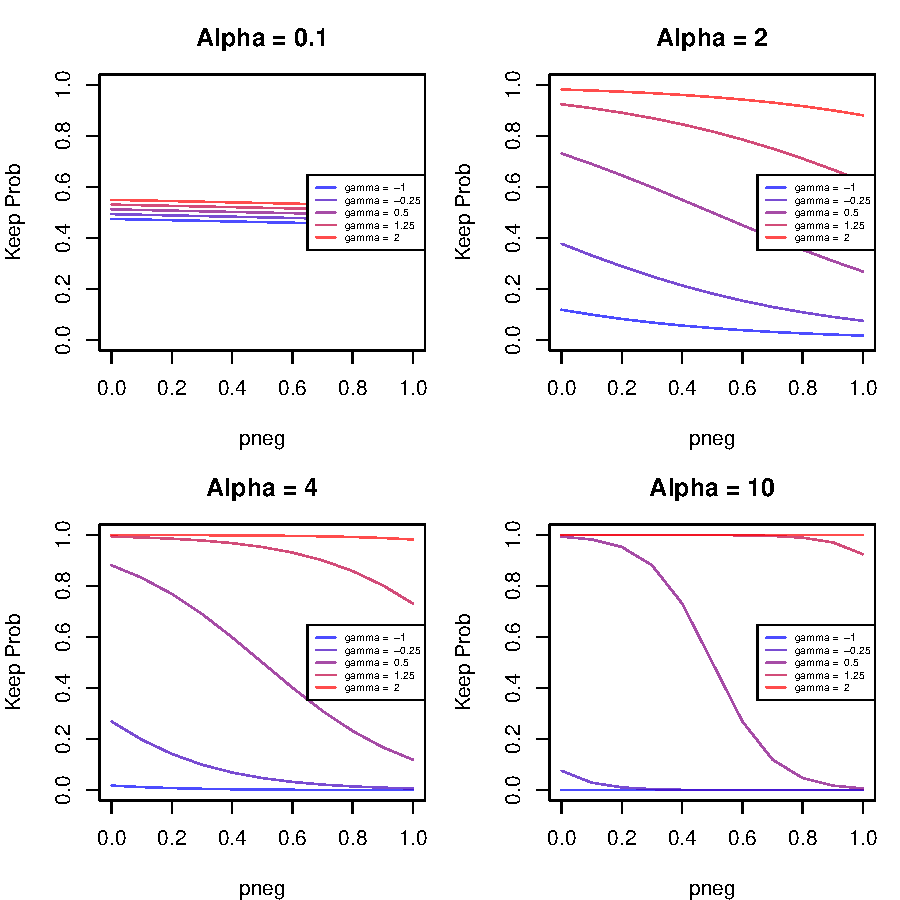
\includegraphics[width=12cm]{keepneg.pdf}
\caption{Probability of keeping as a function of the perceived probability of obtaining a negative sample (pneg), sensitivity to perceived differences in the probability of obtaining a negative outcome (gamma), and overall bias towards keeping (alpha).}
\label{fig:actionpneg}
\end{figure}
\end{center}


\subsubsection{Expectations}

The second action function predicts that people will keep an option as an increasing function of the expectations of options. The model has two parameters: $\alpha$, which dicates the expectation value at which people are equally likely to peek or keep, and $\gamma$, the degree to which people are deterministic in their decision to peek or keep for a given expectation.

\begin{center}
\begin{equation}
\label{eq:actionexpectation}

Pr(Keep_{t})= \frac{1}{1 + e^{-(E_{j} - \alpha} \times \gamma}}

\end{equation}
\end{center}

$E_{j}$ falls in the range [-Inf, Inf] and is the expectation of option j at the current trial. $\alpha$ falls in the range [-Inf, +Inf], and is the indifference point (the expectation value at which the person is equally likely to peek or keep). As $\alpha$ increases, people are generally more likely to peek. $\gamma$ falls in the range [0, +Inf] and is the sensitivity to differences in expectations close to the indifference point. As $\gamma$ increases, people are much more deterministic in their decision to peek or keep. A graph of this function is presented in Figure~\ref{fig:actionexp}



\begin{center}
\begin{figure}
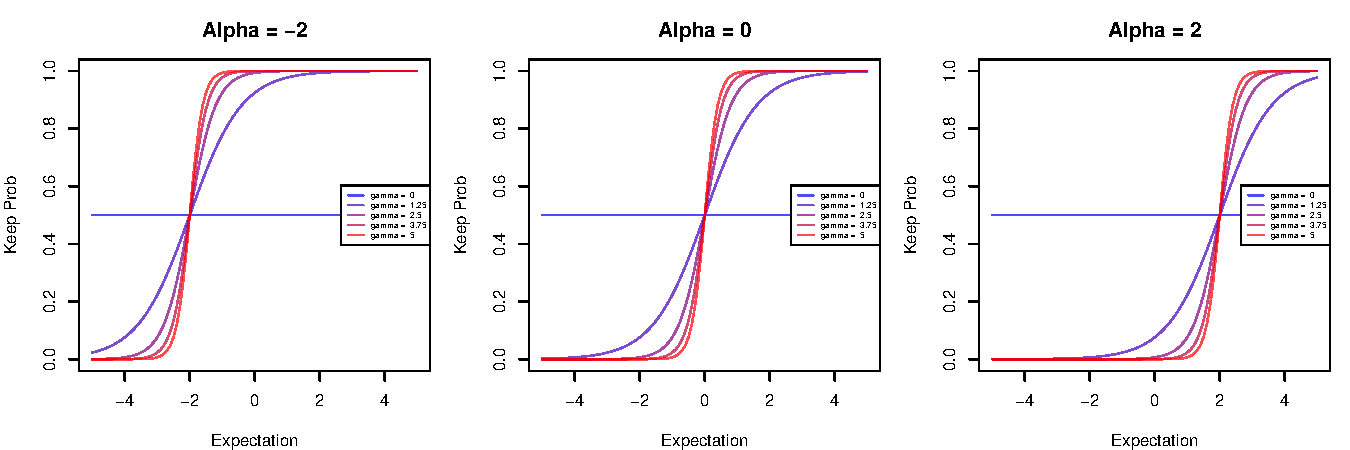
\includegraphics[width=12cm]{keepexp.pdf}
\caption{Probability of keeping as a function of the expectation of an option (exp), an overall bias towards keeping (alpha), and choice consistency (gamma)}
\label{fig:actionexp}
\end{figure}
\end{center}


\subsubsection{Uncertainty}

The third action function predicts that people will keep an option as decreasing function of the uncertainty associated with the option. We define uncertainty in one of 3 ways

\begin{itemize}
  \item Sample standard deviation
  \item Number of prior samples of the option
  \item Standard error of the option
\end{itemize}

The three models corresponding to each of these measures of uncertainty each have one parameter: $\alpha$, which dicates recency effects. As $\alpha$ increases, participants are increasingly more sensitive to recent outcomes in their action decisions. Like models of expectation updating (see future section), we assume that people update their measures of uncertainty as a weighted function of their previous uncertainty measure and new values:

\begin{center}
\begin{equation}
\label{eq:uncertaintyupdatingmodels}

U_{j}(t)=U_{j}(t-1)+\alpha \times [y(t) - U_{j}(t-1)]

\end{equation}
\end{center}

where $U_{j}{t}$ is the uncertainty at trial t, $U_{j}(t-1)$ is the uncertainty on the previous trial, y(t) is the observed uncertainty at trial j, and $\alpha$ is the recency parameter.

The definition of $y(t)$ depends on the specific definition of uncertainty


\subsection{Updating}

After an option has been selected and acted upon, the decision maker updates her expectations of the selected option. We follow previous research \citep{yechiam2005models} and assume that expectations are updated as a function of prior expectations and the newly observed value:

\begin{center}
\begin{equation}
\label{eq:updating}

E_{j}(t)=E_{j}(t-1)+\alpha \times [v(t) - E_{j}(t-1)]

\end{equation}
\end{center}

where $\alpha$ is the updating parameter with a support of [0, 1]. When $\alpha$ is close to 0, expectations do not change much after each observation. When $\alpha$ is close to 1, expectations are strongly influenced by recent outcomes.

We leave open the possibility for different values of $\alpha$ for different actions. For example, one could have a large recency effect and fast updating for keep actions, and low recency effects and slow updating for peek actions. We will test these assumptions in our data.

\subsection{Action-Selection-Updating Model}

The ASU model assumes that people can be in one of two mutually exclusive action states: exploration or exploitation. When people are in an exploration state, they only peek and when they are in an exploitation state they only keep. The probability that people are in an exploration state depends on the current trial and the time since their previous exploration state. We assume that people are more likely to be in an exploration state on earlier trials than later trials, and that people are increasingly more likely to be in an exploitation state the longer it has been since their last exploitation state.

Formally, we define the probability of being in an exploration state as follows. Let $S(t)$ be the state of the decision maker on trial t, where $S(t) \epsilon (0, 1)$ Additionally, let $\beta$ be the number of trials since the last state change.

If the decision maker is in state 1 on trial t - 1, then the probability that he will switch to an exploration state 0 on trial (t) is giving by

\begin{center}
\begin{equation}
\label{eq:modeswitch}

Pr(S(t)=0|S(t-1) = 1)= \frac{1}{1 + e^{-t \times \gamma - \beta}}

\end{equation}
\end{center}

where t is the current trial number, $\beta$ is the number of trials since the previous observation state. 

\begin{knitrout}
\definecolor{shadecolor}{rgb}{0.969, 0.969, 0.969}\color{fgcolor}
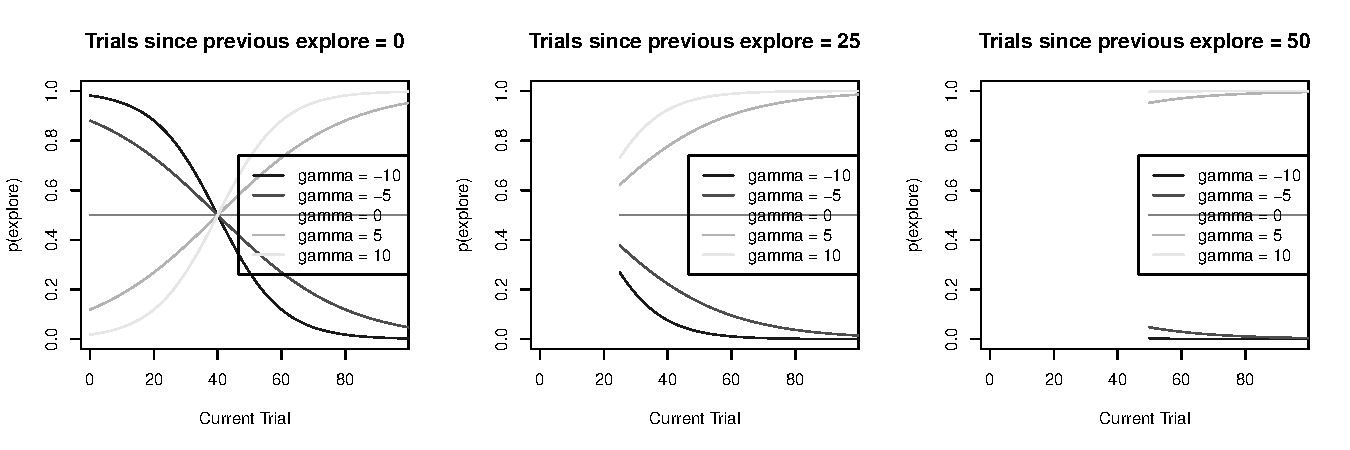
\includegraphics[width=\maxwidth]{figure/unnamed-chunk-5-1} 

\end{knitrout}


If you are currently in an exploration state on trial (t-1), then the probability you will switch to an exploitation state on trial (t) is giving by

\begin{center}
\begin{equation}
\label{eq:modeswitch2}

Pr(State=Exploit{t} | Previous state is explore)= 1-\frac{1}{1 + e^{-runs \times \gamma}}

\end{equation}
\end{center}

































\bibliography{/Users/Nathaniel/Dropbox/Nathaniel_BibTek}
\end{document}
